\documentclass[10pt,aspectratio=169]{beamer}
\usepackage[utf8]{vietnam}
\usepackage{fil}

\title{Mô phỏng thuật toán Reinforcement Learning cho Serverless}
\subtitle{Future Internet Laboratory}
\author{Nguyễn Phạm Trung Hiếu}

\begin{document}

\maketitle

\begingroup
    \begin{frame}{Nội dung chính}{}
        \tableofcontents
    \end{frame}
\endgroup

\section{Chi tiết mô phỏng}

\subsection{Kịch bản mô phỏng}

\begin{frame}{Kịch bản mô phỏng}
\begin{itemize}
\setlength\itemsep{8pt}
\item Hệ thống khởi tạo ngẫu nhiên số lượng container và thời gian xử lý request ở mỗi service.
\item Hệ thống có số service là 4 (\keyword{\textcolor{mainblue}{\lstinline{size = 4}}}), tức ma trận container có 4 hàng.
\item Hệ thống nhận request vào mỗi $ \Delta t = 10s $, thời gian tồn tại của request là $ 2s $.
\item Mỗi 1 giây, hệ thống sẽ tính toán reward và các giá trị info (lượng RAM sử dụng, năng lượng tiêu thụ, profit...).
\item Mỗi 1 giây, thực hiện kiểm tra lượng container ở trạng thái WarmCPU có trong mỗi service và so sánh với lượng request:
\begin{itemize}
\setlength\itemsep{4pt}
\item[-] Nếu $ n_{WarmCPU} \geq n_{request} $ thì $ n_{WarmCPU} -= n_{request} $ rồi đặt $ n_{request} = 0 $, sau đó chờ thời gian xử lý, tính toán các tham số đánh giá, rồi cộng trở lại lượng WarmCPU vừa trừ.
\item[-] Nếu $ n_{WarmCPU} < n_{request} $ thì $ n_{request} -= n_{WarmCPU} $ rồi đặt $ n_{WarmCPU} = 0 $, lượng request dư ra được đưa vào hàng chờ, sau đó xử lý tương tự như trường hợp trên.
\end{itemize}
\end{itemize}
\end{frame}

\begin{frame}{Điều kiện dừng}{\subsecname}
\begin{itemize}
\setlength\itemsep{8pt}
\item Khi hệ thống chạy được một khoảng thời gian là \keyword{\textcolor{mainblue}{\lstinline{container_lifetime = 43200}}},
\item Hoặc thiếu tài nguyên (phần trăm sử dụng CPU hay GPU lớn hơn 1),
\item Hoặc xảy ra hiện tượng tràn RAM...
\end{itemize}
\end{frame}

\begin{frame}{Điều kiện thay đổi trạng thái}{\subsecname}
\begin{itemize}
\setlength\itemsep{8pt}
\item Giới hạn sự thay đổi state chỉ giữa hai state liền kề, state chỉ thay đổi một mức mỗi lần.
\item Biểu diễn ma trận đơn vị $ M_u $ theo cách hiểu khác (nói thêm ở vấn đề gặp phải):
\begin{itemize}
\setlength\itemsep{4pt}
\item[-] -1: state nguồn, tương ứng với state bị thay đổi
\item[-] 1 : state đích, tương ứng với state thay đổi tới
\item[-] 0 : state không bị thay đổi
\end{itemize}
\item[] $ \longrightarrow $ Hai giá trị -1 và 1 luôn liền kề nhau (nếu có thay đổi ở hai vị trí state thì -1 và 1 sẽ được xếp theo từng cặp).
\end{itemize}
\end{frame}

\begin{frame}{Điều kiện thay đổi trạng thái}{\subsecname}
\begin{center}
\textbf{\small Trường hợp thoả mãn}\\
\vspace{4pt}
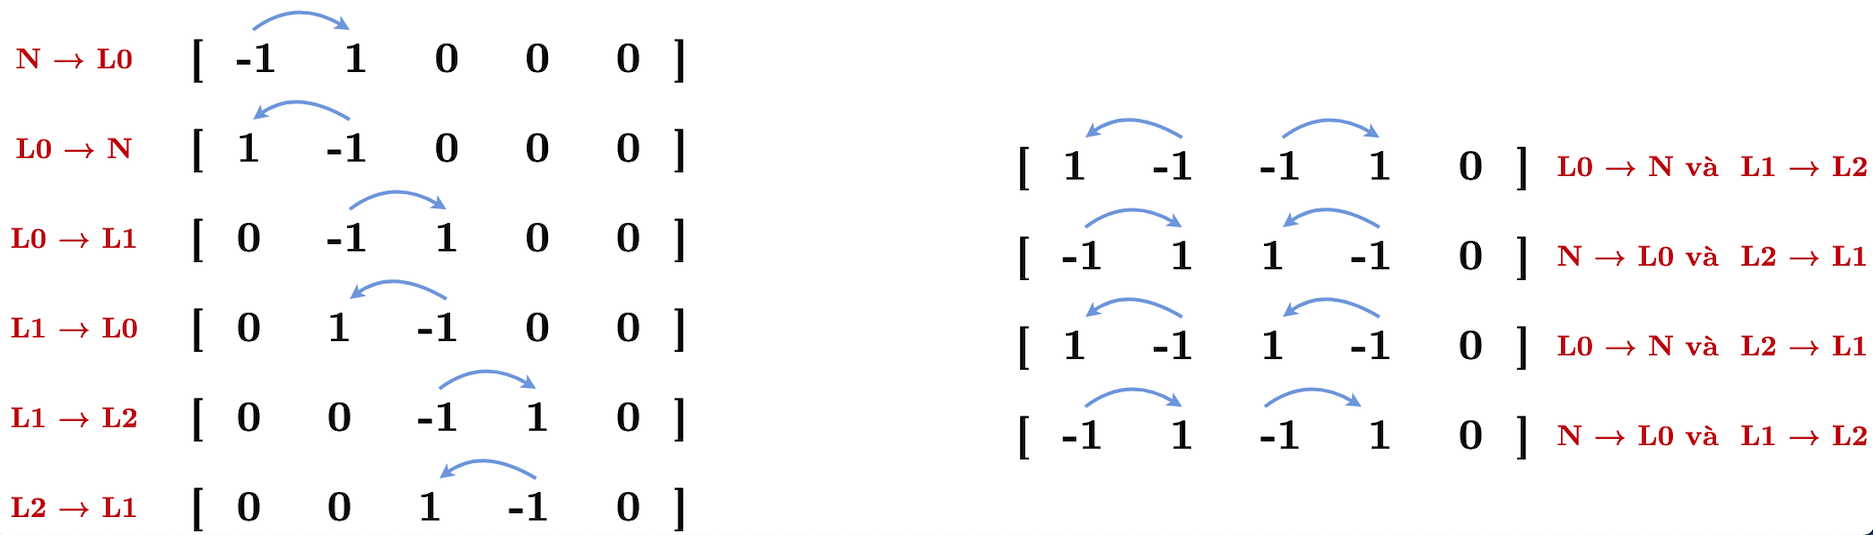
\includegraphics[width=0.8\textwidth]{source/1.png}\\
\vspace{8pt}
\textbf{\small Trường hợp không thoả mãn}\\
\vspace{2pt}

\includegraphics[width=0.6\textwidth]{source/2.png}\\
\end{center}
\end{frame}

\subsection{Mô hình hoá trình mô phỏng}

\begin{frame}{Quy trình mô phỏng}{\subsecname}
\begin{center}
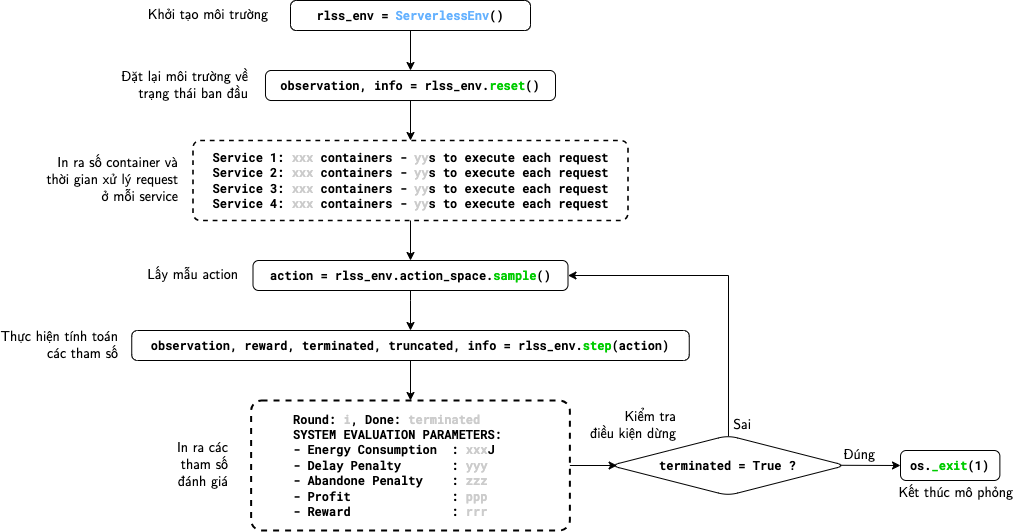
\includegraphics[width=0.88\textwidth]{source/3.png}\\
\end{center}
\end{frame}

\begin{frame}{Mối liên hệ giữa các hàm}{\subsecname}
\begin{center}
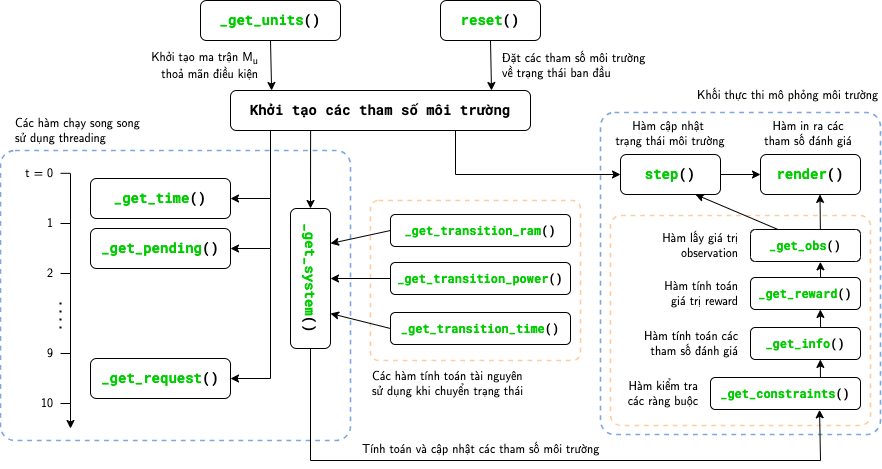
\includegraphics[width=0.86\textwidth]{source/4.png}\\
\end{center}
\end{frame}

\subsection{Triển khai các tham số môi trường}

\begin{frame}[fragile]{Triển khai các tham số môi trường}
Các tham số chính của môi trường:\\
\vspace{8pt}
\scriptsize
\begin{lstlisting}[language=Python]
    self.size = size  # The number of services
    self.num_states = 5  # The number of states in a container's lifecycle
    self.num_resources = 3  # The number of resource parameters (RAM, GPU, CPU)
    self.min_container = 16
    self.max_container = 256
        
    self.timeout = 2  # Set timeout value = 2s
    self.container_lifetime = 43200  # Set lifetime of a container = 1/2 day
    self.limited_ram = 64  # Set limited amount of RAM (server) = 64GB
    self.limited_request = 128
\end{lstlisting}
\end{frame}

\begin{frame}[fragile]{Triển khai các tham số môi trường}
Không gian observation và action của môi trường:\\
\vspace{8pt}
\tiny
\begin{lstlisting}[language=Python]
self.observation_space = spaces.Dict({
    "execution_times":   spaces.Box(low=1,high=10, shape=(self.size, 1), dtype=np.int16),
    "request_quantity":  spaces.Box(low=0,high=self.limited_request, shape=(self.size, 1),dtype=np.int16),
    "remained_resource": spaces.Box(low=0,high=self.limited_ram, shape=(self.num_resources, 1),dtype=np.int16),
    "container_traffic": spaces.Box(low=0,high=self.max_container, shape=(self.size, self.num_states),dtype=np.int16),
})
        
self._action_coefficient = spaces.Box(low=0, high=0, shape=(self.size, self.size), dtype=np.int16)
self._action_unit = spaces.Box(low=-1, high=1, shape=(self.size, self.num_states), dtype=np.int16)
self.action_space = spaces.Tuple((self._action_coefficient, self._action_unit))
        
# Set the main diagonal elements of _action_coefficient to be in the range [0, self.max_container] 
np.fill_diagonal(self._action_coefficient.low, 0)
np.fill_diagonal(self._action_coefficient.high, self.max_container)
        
# Set the last column of _action_unit to be always zero and the sum of the elements in a row of _action_unit = 0
self._get_units()
\end{lstlisting}
\end{frame}

\begin{frame}[fragile]{Triển khai các tham số môi trường}
Một số tham số và ma trận khởi tạo khác:\\
\vspace{8pt}
\scriptsize
\begin{lstlisting}[language=Python]
    self.current_time = 0  # Start at time 0
    self.transition_ram = 0 
    self.transition_time = 0
    self.transition_power = 0 
    self._custom_request = np.random.randint(0, 64, size=(self.size, 1))
    self._pending_request = np.zeros((self.size, 1), dtype=np.int16) 
    self._ram_required_matrix = np.array([0, 0, 0, 0.9, 2])
    self._action_matrix = np.zeros((self.size, self.num_states), dtype=np.int16) 
    self._exectime_matrix = np.random.randint(2, 16, size=(self.size, 1))
    self._request_matrix = np.zeros((self.size, 1), dtype=np.int16)
    self._resource_matrix = np.ones((self.num_resources, 1), dtype=np.int16)
    self._resource_matrix[0, 0] = self.limited_ram
    self._container_matrix = np.hstack((
        np.random.randint(self.min_container, self.max_container, size=(self.size, 1)),
        np.zeros((self.size, self.num_states-1), dtype=np.int16)
    )) 
\end{lstlisting}
\end{frame}

\section{Triển khai mô phỏng và đánh giá}

\subsection{Kết quả mô phỏng}

\begin{frame}{Kết quả mô phỏng}
\begin{center}
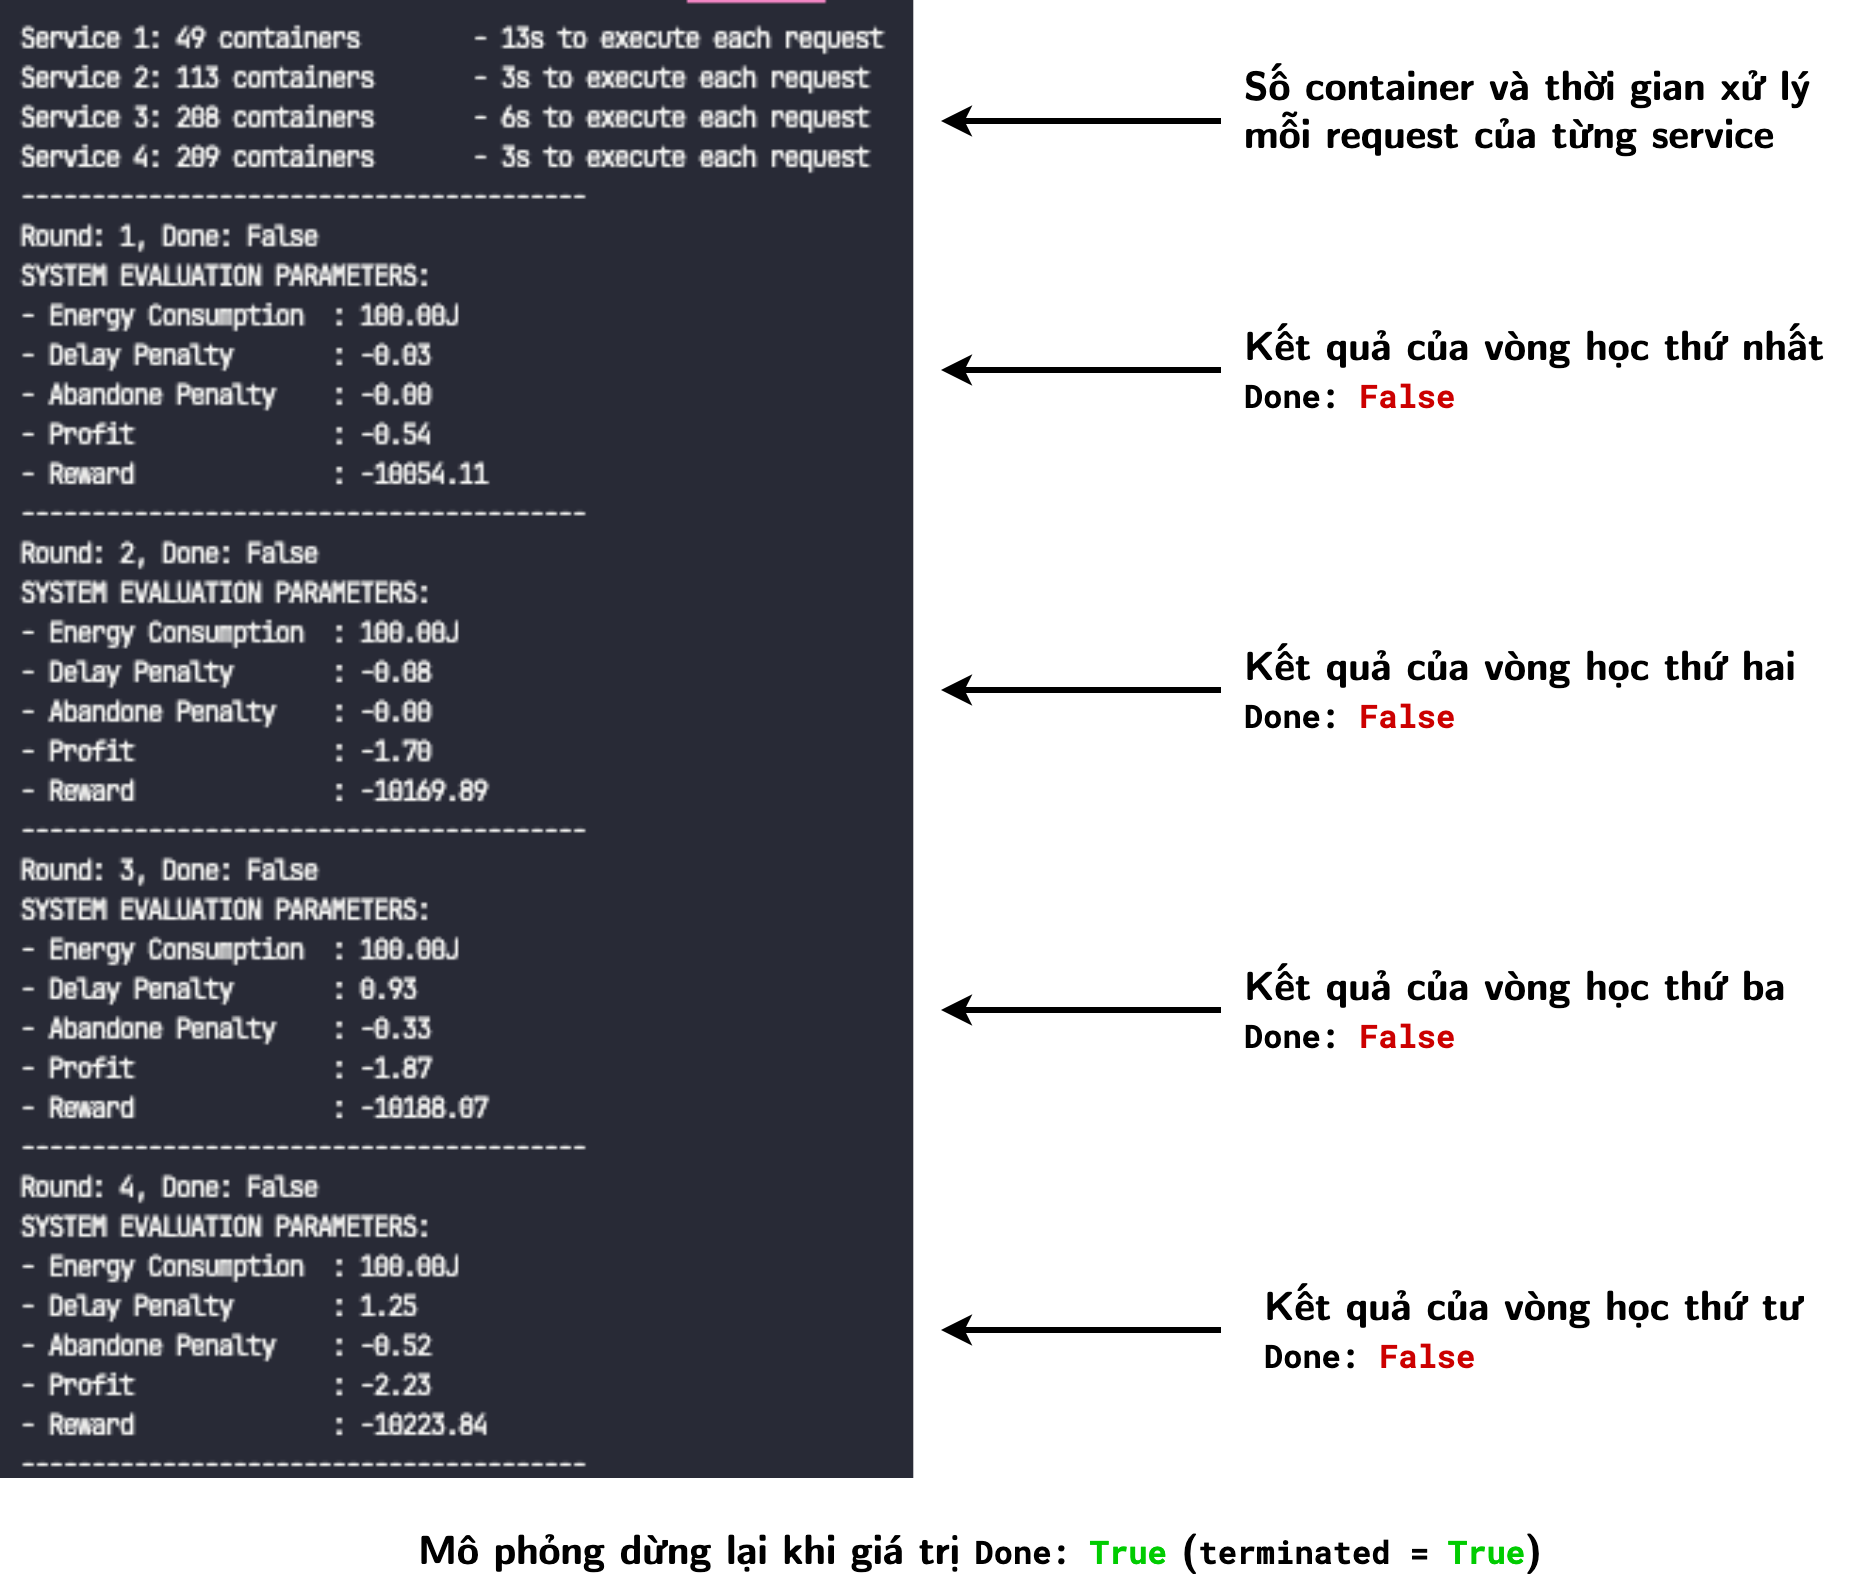
\includegraphics[width=0.54\textwidth]{source/5.png}\\
\end{center}
\end{frame}

\subsection{Đánh giá mô phỏng}

\begin{frame}{Nhận xét kết quả}{\subsecname}
\begin{itemize}
\setlength\itemsep{8pt}
\item Kết quả reward nhận được bị âm, giảm dần qua các vòng học
\item[] $ \longrightarrow $ \textbf{Nguyên nhân:} Hệ số $ a $ và $ b $ trong công thức tính reward đang đặt là 100.
\begin{equation*}
Reward = a \times Profit - b \times Energy_{cost} - Penalty_{delay} - Penalty_{abandone}
\end{equation*}
\item Đôi lúc mô phỏng chỉ chạy được 1-2 vòng học rồi dừng lại.
\item[] $ \longrightarrow $ \textbf{Nguyên nhân:} Điều kiện xác định \keyword{\textcolor{mainblue}{\lstinline{terminated}}} chưa chặt chẽ, hoặc do lập trình sai.
\item Kết quả mô phỏng chưa đánh giá được vấn đề cho bài toán, vì chưa kết hợp hệ thống mô phỏng request đến mà chỉ mới cho random, hoặc do lập trình sai.
\end{itemize}
\end{frame}

\begin{frame}{Vấn đề gặp phải (1)}{\subsecname}
\textbf{Ví dụ:}
\begin{center}
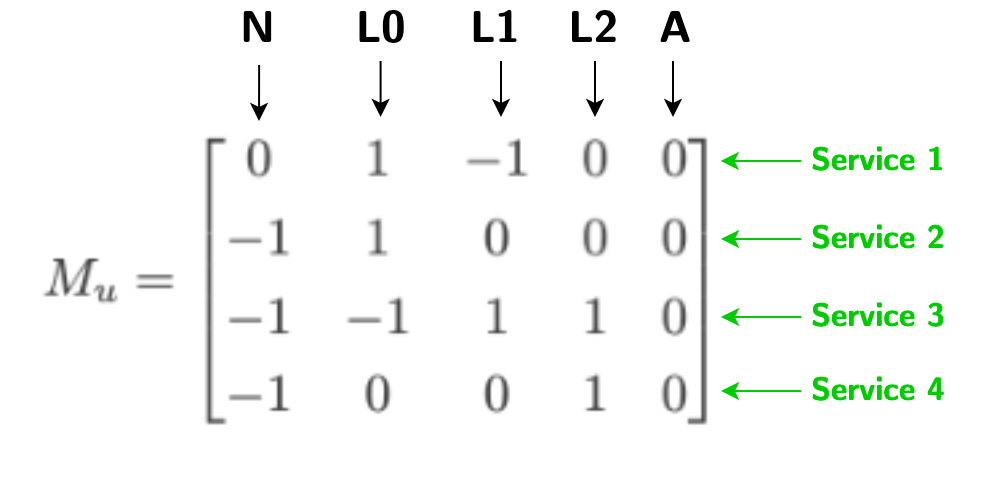
\includegraphics[width=0.52\textwidth]{source/6.png}
\end{center}
\scriptsize
\begin{itemize}
\setlength\itemsep{8pt}
\item Đối với ma trận đơn vị $ M_u $, ta có các phần tử $ u_{ij}\,\epsilon\,\{ -1, 0, 1\}$ lần lượt là các action quay state trước đó, không thay đổi state và chuyển đến state kế tiếp.
\item Đối với service 1, giả sử ta có $ x_1 $ container đang ở trạng thái L0 sẽ được chuyển đến state kế tiếp, và $ x_1 $ container đang ở trạng thái L1 sẽ được chuyển về state trước đó.
\end{itemize}
\end{frame}

\begin{frame}{Vấn đề gặp phải (1)}{\subsecname}
\textbf{Ví dụ:}
\small
\begin{itemize}
\setlength\itemsep{8pt}
\item Khi đó, khi cập nhật ma trận state $ M_{s+1} = M_s + M_a $, giả sử có sẵn 50 container ở L0 và 40 container ở L1, thì số container sau khi cập nhật sẽ thành $ (50 + x_1) $ L0 và $ (40 - x_1) $ L1.
\item[] $ \rightarrow $ Chỉ hiểu được $ x_1 $ container chuyển từ L1 về L0, còn phần chuyển đến state kế tiếp của L0 thì không thể hiện được.
\item[] $ \rightarrow $ Vấn đề xảy ra tương tự với service 2 và service 4.
\item Ở service 3, không thể xác định được container chuyển từ state nào đến state nào?
\item[] $ \rightarrow $ Việc tính toán các tham số đánh giá nếu chuyển nhiều state trong một \keyword{\textcolor{mainblue}{\lstinline{step}}} rất khó khăn.
\end{itemize}
\normalsize
$ \longrightarrow $ \textit{Đề xuất đặt các điều kiện như kịch bản mô phỏng.}
\end{frame}

\begin{frame}{Vấn đề gặp phải (2)}{\subsecname}
\begin{itemize}
\setlength\itemsep{8pt}
\item Tính $ Penalty_{delay} $ và $ Penalty_{abandone} $ chưa đúng? Hiểu sai? (Cần hỏi lại)
\item Tính toán năng lượng $ Energy_{cost} $ chưa đúng? Lập trình sai?
\item Tính toán các tham số chuyển state chưa đúng?
\end{itemize}
\end{frame}

\section{Kết luận}

\begin{frame}{Kết luận}
\begin{itemize}
\setlength\itemsep{8pt}
\item Link Github mô phỏng: \textit{
\href{https://github.com/owofuyuki/reinforcement-learning-for-serverless}{https://github.com/owofuyuki/reinforcement-learning-for-serverless}}
\item Kết quả mô phỏng chưa đánh giá được vấn đề cho bài toán, vì chưa kết hợp hệ thống mô phỏng request đến mà chỉ mới cho random, hoặc do lập trình sai.
\item Chỉnh sửa mô phỏng...
\end{itemize}
\end{frame}

\backmatter

\end{document}